\documentclass[a4paper]{report}

%====================== PACKAGES ======================

\usepackage[french]{babel}
\usepackage[utf8]{inputenc}
%pour gérer les positionnement d'images
\usepackage{float}
\usepackage{amsmath}
\usepackage{graphicx}
\usepackage[colorinlistoftodos]{todonotes}
\usepackage{url}
%pour les informations sur un document compilé en PDF et les liens externes / internes
\usepackage{hyperref}

%espacement entre les lignes
\usepackage{setspace}
%modifier la mise en page de l'abstract
\usepackage{abstract}
%police et mise en page (marges) du document
\usepackage[T1]{fontenc}
\usepackage[top=2cm, bottom=2cm, left=2cm, right=2cm]{geometry}
%Pour les galerie d'images
\usepackage{subfig}

%====================== INFORMATION ET REGLES ======================

%rajouter les numérotation pour les \paragraphe et \subparagraphe
\setcounter{secnumdepth}{4}
\setcounter{tocdepth}{4}

%======================== DEBUT DU DOCUMENT ========================

\begin{document}

\tableofcontents
\thispagestyle{empty}
\setcounter{page}{0}
%ne pas numéroter le sommaire

\newpage



%====================== INCLUSION DES PARTIES ======================





\chapter{Réalisation}

\section{Problèmes rencontrés durant le projet}
\begin{spacing}{2}
\par 
Durant la réalisation du projet, nous avons rencontré des problèmes dont les unes sont plus graves que les autres. Nous avons pu trouver des solutions à certaines problèmes mais il restait des problèmes sans solution qui ont retardé l'avancement de notre projet. Je les cite comme suit :
\begin{itemize}
\item[•] \textbf{Implémentation des API :} nous avons trouvé du mal à introduire les API surtout celles du Google Maps et du Facebook. Des contraintes de paiement et de restrictions ont été imposées, ce qui a limité les fonctionnalités de notre projet : nous avons réussi à implémenter l'API du Facebook mais très limité. 
\item[•] \textbf{Implémentation du Chat Bot:} le déploiement du Chat Bot dans notre application n'a pas été possible parce que la dependency correspondante au Chat Bot n'a pas été identifiée correctement.
\item[•] \textbf{Upload des images dans les profils des utilisateurs :} problème de chargement de l'image au premier accès à l'espace de l'utilisateur.
\item[•] \textbf{Différentes configurations sur un le même projet:} nous avons adopté les solutions cherchées sur Internet mais ça n'a pas marché. 
\end{itemize} 

\par
Pour toute référence et détails sur un problème , veuillez accéder à notre projet sur GitHub dans la sections Issues. 
\cleardoublepage
\begin{figure}[!ht]
\begin{center}
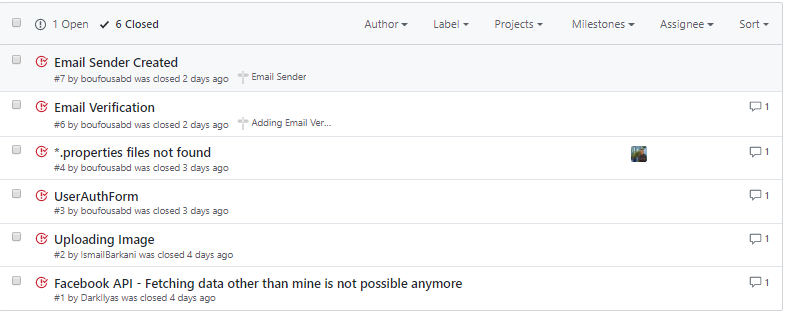
\includegraphics[height=6cm]{issues.png}
\end{center}
\caption[Section Issues du projet]{Section Issues du projet\protect\footnotemark}
\end{figure}
\footnotetext{lien vers la section Issues du projet https://github.com/ENSIAS-MEH/Wasselni--Platforme-de-covoiturage-JEE-/issues } 

\end{spacing}
\end{document}